\documentclass[11pt]{article}
\usepackage[margin=4mm]{geometry}
\usepackage[absolute]{textpos}
\usepackage{expl3}
\usepackage{xparse}
\usepackage{parskip}
\usepackage{setspace}
\usepackage[normalem]{ulem}
\usepackage{fontspec}
\usepackage[skins,hooks]{tcolorbox}
\usepackage{xcolor}
\usepackage{metalogo}
\usepackage{listings}
\usepackage{microtype}
\usepackage{array}
\usepackage{graphicx}
\usepackage{amssymb}
\usepackage{enumitem}
\usepackage{tikz}
\usepackage{vwcol}
\usepackage[hidelinks]{hyperref}

\definecolor{c-headerupper}{HTML}{9C9687}
\definecolor{c-headerlower}{HTML}{b2a25c}
\definecolor{c-text-white}{HTML}{ffffff}
\definecolor{c-text-primary}{HTML}{000000}
\definecolor{c-text-secondary}{HTML}{ceb888}
\definecolor{c-skill-gray}{HTML}{a0a0a0}


\newlength{\headerheight}
\makeatletter
\ExplSyntaxOn
\tcbset{
    headerbox/.style={
        bicolor,
        width=\paperwidth, 
        nobeforeafter, 
        boxrule=0pt, 
        frame~hidden, 
        arc=0mm,
        colback=c-headerupper,
        colbacklower=c-headerlower,
        left=1.5cm,
        right=1.5cm,
        top=5mm,
        frame~code~app={
            \dim_gset:Nn \headerheight {\tcb@innerheight}
        }
    }
}

\DeclareDocumentEnvironment{header}{+b}{
    \begin{textblock*}{\paperwidth}(0pt,0pt)%
    #1%
}{
    \end{textblock*}
    \vspace*{\headerheight}
}


\DeclareDocumentEnvironment{triplehead}{mmm}{
\par {\large\bfseries #1}
\par #2
\par {\color{c-text-secondary}\itshape\small #3}
\par\smallskip
}{\par\medskip}

\tcbset{
    skillbarbox/.style={
        colback=c-text-secondary,
        nobeforeafter,
        height=1em,
        left=0em,
        right=0em,
        top=0em,
        bottom=0em,
        boxsep=0em,
        frame~hidden,
        boxrule=0pt
    }
}

\newcommand{\skillbar}[1]{
    \regex_split:nnN {/} {#1} \l_tmpa_seq
    \exp_args:Nx \int_set:Nn \l_tmpa_int {\seq_item:Nn \l_tmpa_seq {1}}
    \exp_args:Nx \int_set:Nn \l_tmpb_int {\seq_item:Nn \l_tmpa_seq {2}}
    \int_step_inline:nn {\l_tmpb_int} {
        \int_compare:nTF {##1 <=\l_tmpa_int} {
            \tcbox[skillbarbox]{\hspace*{1em}}\hspace{1ex}
        } {
            \tcbox[skillbarbox, colback=c-skill-gray]{\hspace*{1em}}\hspace{1ex}
        }
    }
}

\cs_set:Npn \cvhead_impl:Nn #1#2 {
    \vspace{2em}{\renewcommand{\ULthickness}{2pt}\color{c-text-secondary}#1\bfseries \uline{\MakeUppercase{#2}}}\par\bigskip
}
\newcommand{\cvhead}[1]{\cvhead_impl:Nn \Large {#1}}
\newcommand{\cvsubhead}[1]{\vspace{1em}{\centering\renewcommand{\ULthickness}{1.5pt}\color{c-text-secondary}\large\bfseries \uline{\scshape #1}\par}\bigskip}

\ExplSyntaxOff
\makeatother

\newfontfamily{\fabrand}{Font Awesome 5 Brands-Regular-400}
\newfontfamily{\faregular}{Font Awesome 5 Free-Regular-400}
\newfontfamily{\fasolid}{Font Awesome 5 Free-Solid-900}
\setsansfont[
Extension=.otf,
BoldFont=texgyreadventor-bold,
ItalicFont=texgyreadventor-italic,
BoldItalicFont=texgyreadventor-bolditalic]{texgyreadventor-regular}
\setmonofont[Extension=.otf]{texgyrecursor-regular}

\renewcommand{\familydefault}{\sfdefault}

\newcommand*{\faemail}{{\fasolid \symbol{"F674}}}
\newcommand*{\falinkedin}{{\fabrand \symbol{"F08C}}}
\newcommand*{\faglobe}{{\fasolid \symbol{"F57D}}}
\newcommand*{\fagithub}{{\fabrand \symbol{"F09B}}}

\setlist[itemize]{left=0pt,label={$\color{c-text-secondary}\blacksquare$}}
\setlist[itemize,2]{label={$\color{c-text-secondary}\bullet$}}

\tcbset{
    skillbox/.style={
        top=0pt,
        bottom=0pt,
        left=1mm,
        right=1mm,
        colframe=c-text-secondary, 
        colback=c-text-secondary,
        nobeforeafter,
        valign=center,
        height=1.6em
    }
}
\newcommand{\skill}[1]{
\tcbox[skillbox]{{\color{c-text-white}#1}}
}

\lstset{
    basicstyle=\ttfamily,
}

\begin{document}

\makeatletter
\begin{header}
\begin{tcolorbox}[headerbox]
% header left
\begin{minipage}{0.75\linewidth}
{\color{c-text-white}\setlength{\parskip}{3pt}
\par{\huge Ziyue ``Alan'' Xiang}
\par {\Large\color{c-text-secondary} Research Assistant}
\par Graduate student researcher with experience in machine learning, specialized in using computer vision approaches to tackle media forensics problems.
}
\par
\end{minipage}\hfill
%header right
\begin{minipage}{0.19\linewidth}
\begin{tikzpicture}
\node[circle, text width=2.8cm, draw, color=c-text-secondary, inner sep=0pt, outer sep=0pt, line width=5pt] at (0, 0) {};
\node at (0, 0) {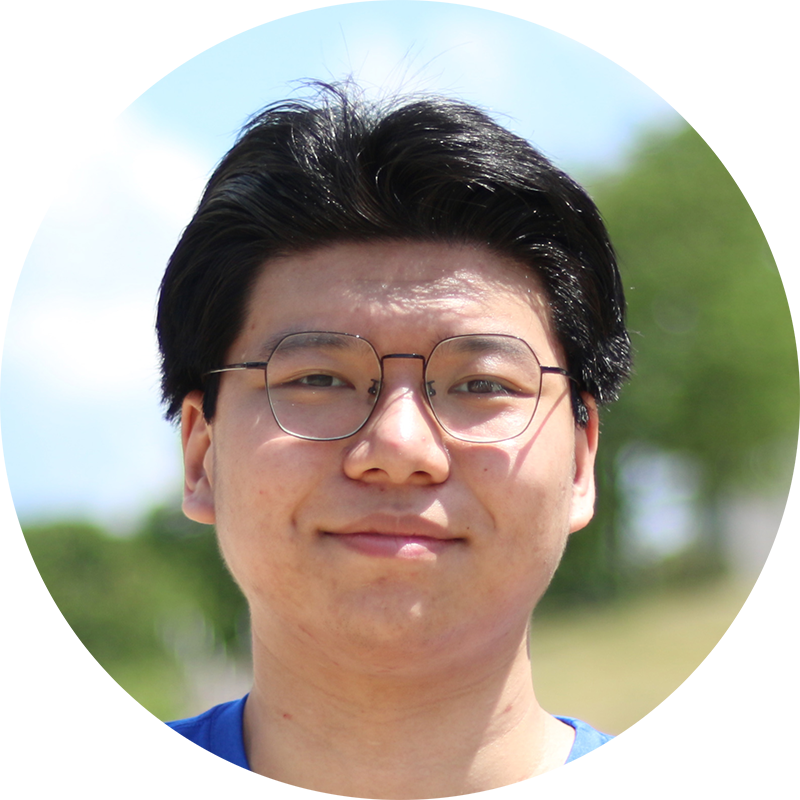
\includegraphics[width=2.8cm]{photo.png}};
\end{tikzpicture}
\end{minipage}
\tcblower
\begin{center}
{\color{c-text-white}\small
\faemail~\href{mailto:xiang71@purdue.edu}{xiang71@purdue.edu}\qquad
\faglobe~\href{https://www.alanshawn.com}{alanshawn.com}\qquad
\falinkedin~\href{https://www.linkedin.com/in/ziyue-alan-xiang/}{ziyue-alan-xiang}\qquad
\fagithub~\href{https://www.github.com/xziyue}{xziyue}
}
\end{center}
\end{tcolorbox}
\end{header}
% main matter
\vspace*{-3em}% adjust spacing
{
\color{c-text-primary}
%left column
\begin{minipage}[t]{0.48\linewidth}
\cvhead{Work Experience}
\begin{triplehead}{Research Assistant}{VIPER Lab, Purdue ECE}{Aug. 2020--Present}
\begin{itemize}
\item Investigating reliable and cost-effective approach to counter deepfake and other types of media forgery technique that may bring substantial threat to the credibility of everyday information
\end{itemize}
\end{triplehead}

\begin{triplehead}{Research Assistant}{SOS+CD Lab, iSchool, Syracuse University}{Aug. 2018--July 2020}
\begin{itemize}
\item Developed automated tools for image manipulation detection in science
\item Assisted the application of US ORI grant: “Human-centered automatic tracing, detection, and evaluation of image and data tampering”
\end{itemize}
\end{triplehead}

\begin{triplehead}{Teaching Assistant}{EECS, Syracuse University}{Jan. 2020--May 2020}
\begin{itemize}
\item Teaching assistant of CIS-375: Discrete Mathematics, lectured by Prof. Andrew C. Lee
\item Participated in grading, hosting office hours, preparing recitation materials
\item Researched and experimented the transition to on-line learning during COVID-19 pandemic
\end{itemize}
\end{triplehead}

\cvhead{Education}

\begin{triplehead}{Ph.D. in Electrical \& Computer Engineering}{Purdue University}{Aug. 2020--Present}
\end{triplehead}

\begin{triplehead}{MSc. in Computer Science}{Syracuse University}{Aug. 2018--May 2020}
\end{triplehead}

\begin{triplehead}{BSc. in Information \& Computing Science}{Sun Yat-sen University, Guangdong, China}{Sept. 2014-June 2018}
\begin{itemize}
\item Best undergraduate thesis award
\end{itemize}
\end{triplehead}

\end{minipage}\hfill
% right column
\begin{minipage}[t]{0.48\linewidth}
\cvhead{Skills}

{\setstretch{1.6}
\par \skill{Data Mining}\skill{Data Visualization}
\par \skill{C++}\skill{Julia}\skill{Lua}\skill{Haskell}
\par \skill{HTML}\skill{CSS}\skill{JavaScript}
\par \skill{Linux security}\skill{Cybersecurity}
\par \skill{tensorflow}\skill{Apache Spark}
\par
}

\cvsubhead{Key Skills}

\begin{itemize}
\item Python
\begin{itemize}
\item Proficient in the usage of numpy and scipy, which maximizes Python's performance
\item Experienced at parallelizing Python, as well as extending Python with Cython or C++
\end{itemize}
\item Machine learning (computer vision)
\begin{itemize}
\item Studied and understood the mathematical derivation of most off-the-shelf machine learning algorithms
\item Familiar with machine learning toolkits (e.g. sckit-learn) and computer vision toolkits (e.g. OpenCV)
\end{itemize}
\item \LaTeX
\begin{itemize}
\item Familiar with advanced \TeX\ technologies such as \LaTeX3 and \LuaLaTeX
\item Active package developer in \LaTeX\ community (e.g. luaprogtable)
\end{itemize}
\end{itemize}

\cvhead{Languages}
{
\renewcommand{\arraystretch}{1.5}
\setlength{\tabcolsep}{0pt}
\begin{tabular}{l<{\hspace{8mm}}l}
English & \skillbar{5/6}\\
Chinese(Mandarin) & \skillbar{6/6}\\
Cantonese & \skillbar{4/6}
\end{tabular}
}

\cvhead{Training\raisebox{2pt}{/}Certificates}
\begin{itemize}
\item Graduate teaching assistant training (2020)
\item CITI Program--Responsible Conduct of Research (2019)
\item CITI Program--Biomedical Research Investigators and Key Personnel
(2020)
\end{itemize}


\end{minipage}
}

\begin{textblock*}{\linewidth}(1cm,4pt)
\footnotesize If you like this template, you can find its source code at \href{https://github.com/xziyue/cv-onepager}{https://github.com/xziyue/cv-onepager}
\end{textblock*}

\end{document}